\begin{figure*}[ht!]
\begin{center}
    \begin{minipage}[b]{1\textwidth}
        \begin{subfigure}[b]{0.475\textwidth}
            \centering
            \includegraphics[scale=0.10]{figures/P26_39-comparison.png}
            \caption{Variation of Baseline Models}
            \label{fig:var_baseline}
        \end{subfigure}\quad
        \begin{subfigure}[b]{0.475\textwidth}
            \centering
            \includegraphics[scale=0.2]{figures/mstcn_howto100m.png}
            \caption{MS-TCN with Joint Embedding}
            \label{fig:mstcn_joint}
        \end{subfigure}
        \caption{Qualitative results of Methods}
        \label{fig:baseline_qualitative}
    \end{minipage}
\end{center}
\end{figure*}

% \begin{figure}[h!]
%   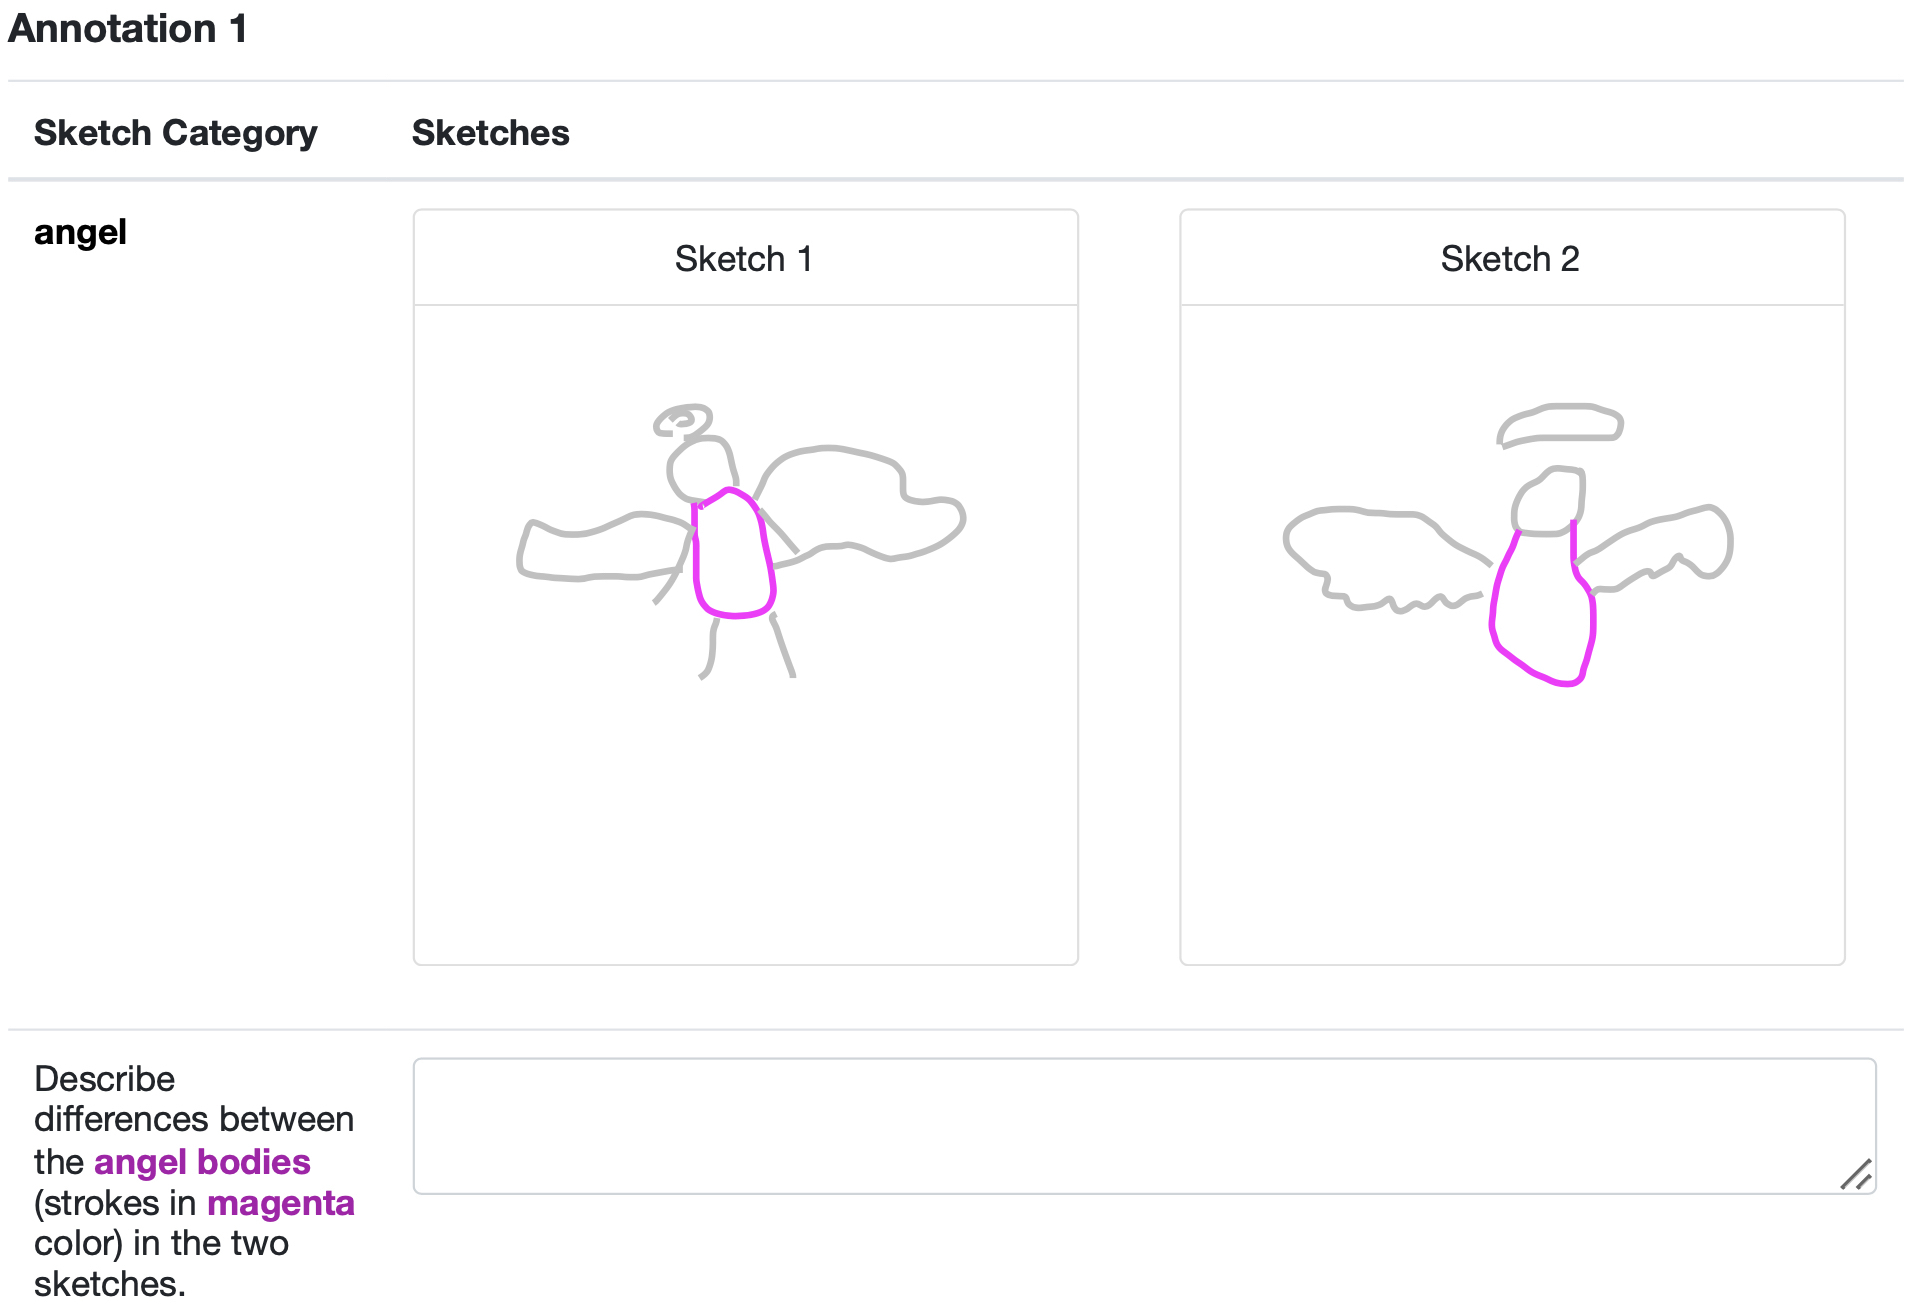
\includegraphics[width=150mm]{version_2/pilot_02_01_annotation_1.png}
%   \caption{The birds The birds The birds The birds The birds The birds The birds The birds The birds The birds}
%   \label{v2.main_task.1}
% \end{figure}

\begin{table*}[h!]
\begin{minipage}[b]{1\textwidth}
\centering
\begin{tabular}{lrrrrrr}
\toprule
% & \multicolumn{3}{c}{Test}\\
Methods  & Acc & Edit & F1$@\{10,25,50\}$ \\
\midrule
FC  & 34.90 & 18.58 & 17.47~~13.66~~8.04\\
% EDTCN \cite{8099596} & & & & & & \\
MS-TCN \cite{8953830} & 38.65 & & \\
% RNN+HMM \cite{8099623} & & & & & & \\
DTGRM \cite{wang2020temporal} & 37.71 & & \\
\midrule
Proposed Method (\textit{narration}) & 20.93 & 24.20 & 2.49 & \\
Proposed Method (\textit{narration+context})& 22.81 & 24.40 & 2.69 & \\
\bottomrule
\end{tabular}
\caption{Results of baseline models}
\label{table:results}
\end{minipage}
~\\
\begin{minipage}[b]{1\textwidth}
\centering
\begin{tabular}{lrrrrr}
\toprule
Label &  Segment Threshold ($l_s$) & MR & R1 & R5 & R10 \\
\midrule
\multirow{3}{*}{Narration} & 0 & 46 & 0.03 & 0.11 & 0.18 \\
 & 1 & 40 & 0.04 & 0.14 & 0.22 \\
 & 3 & 13 & 0.10 & 0.30 & 0.45 \\
\midrule
 & 1 & 132 & 0.01 & 0.03 & 0.05 \\
Verb+Context & 3 & 104 & 0.01 & 0.04 & 0.07 \\
 & 5 & 26 & 0.03 & 0.13 & 0.24\\
\midrule
 & 1 & 6 & 0.19 & 0.49 & 0.66 \\
Narration+Context & 3 & 5 & 0.23 & 0.54 & 0.70 \\
 & 5 & 2 & 0.36 & 0.81 & 0.92 \\
\bottomrule
\end{tabular}
\caption{Results of Video-Text Retrieval using different segment threshold}
\label{table:howto100m_seg_threshold}
\end{minipage}
~\\
\begin{minipage}[b]{1\textwidth}
\centering
% \begin{tabular}{lrrrrr}
\begin{tabular}
{c{0.2\linewidth}  c{0.15\linewidth} c{0.08\linewidth} c{0.08\linewidth}  c{0.08\linewidth}  c{0.08\linewidth}}
\toprule
Visual Context Threshold ($l_v$) & Segment Threshold ($l_s$) & MR & R1 & R5 & R10 \\
\midrule
2 & 0 & 135 & 0.01 & 0.03 & 0.07 \\
3 & 0 & 50 & 0.02 & 0.08 & 0.16 \\
4 & 0 & 26 & 0.03 & 0.16 & 0.27 \\
3 & 1 & 36 & 0.03 & 0.14 & 0.23 \\
3 & 3 & 102 & 0.02 & 0.09 & 0.14 \\
\bottomrule
\end{tabular}
\caption{Results of Video-Text Retrieval using different segment threshold on visual features}
\label{table:howto100m_visual_seg_threshold}
\end{minipage}
\end{table*}


\begin{table}[ht!]
\begin{minipage}{1\textwidth}
\begin{center}
{\small
\begin{tabular}{lrrrrrrrr}
\toprule
& \multicolumn{4}{c}{Training} & \multicolumn{4}{c}{Validation}\\
~ & Max. & Min. & Avg. & Std. & Max. & Min. & Avg. & Std. \\
\midrule
Verb class frequency & 14848 & 73 & 1314 & 2829 & 1937 & 71 & 191 & 398\\
Noun class frequency & 3617 & 178 & 724 & 655 & 430 & 25 & 108 & 92\\
Sentence length & 77 & 3 & 15.1 & 6.3 & 71 & 3 & 14.8 & 6.0\\
Actions per video & 940 & 1 & 136 & 168 & 564 & 3 & 70 & 93\\
Frames per verb class & 2129212 & 20165 & 225170 & 408408 & 407425 & 2702 & 42016 & 76950 \\
Video length & 3708 & 10 & 543 & 645 & 1969 & 11 & 344 & 377 \\
\bottomrule
\end{tabular}}
\caption{Statistics of EPIC-KITCHENS-100 training and validation set}
\label{table:train_val_stats}
\end{center}
\end{minipage}
\end{table}


